\chapter{ Технологический раздел}
\label{cha:technological}

    В данном разделе будут выбраны средства реализации ПО и представлен листинг кода. 

    \section{Средства реализации}
        В данной работе используется язык программирования python \cite{c-sharp}, так как
        он позволяет написать программу в относительно малый срок.
        В качестве среды разработки использовался Jupyter Notebook.

        Для замера процессорного времени была использована функция process\_time модуля time.
        Она возвращает значение в долях секунды суммы системного и пользовательского процессорного времени текущего процесса и 
        не включает время, прошедшее во время сна.

    \section{Листинг программы}
        Ниже представлены листинги кода алгоритмов поиска слова в словаре:
        \begin{enumerate}
            \item полным перебором (листинг \ref{lst:brute-force});
            \item бинарным поиском (листинг \ref{lst:binary});
            \item поиском по сегментам (листинг \ref{lst:segment}).
        \end{enumerate}
        
        \begin{lstlisting}[language=python, label=lst:brute-force, caption=Реализация алгоритма поиска слов в словаре полным перебором]
class BruteForceDictionary:
    "Словарь с поиском ключа перебором"
    def __init__(self):
        self.data = []
    
    def keys(self):
        return list(self.__iter__())

    def __getitem__(self, key : str) -> int:
        i = self.__get_index_key(key)
        if i > -1:
            return self.data[i][1]
        return None

    def __setitem__(self, key: str, value: int):
        i = self.__get_index_key(key)
        if i < 0:
            self.data.append((key, value))
        else:
            self.data[i] = (key, value)

    def __contains__(self, key: str):
        return self.__get_index_key(key) > -1

    def __iter__(self):
        return iter(map(lambda pair: pair[0], self.data))

    def __get_index_key(self, key: str) -> int:
        i = 0
        for i, pair in enumerate(self.data):
            if pair[0] == key:
                return i
        return -i - 1
        \end{lstlisting}

        \begin{lstlisting}[language=python, label=lst:binary, caption=Реализация алгоритма двоичного поиска слова в словаре]
class BinarySearchDictionary:
    "Словарь с двоичным поиском ключа"
    def __init__(self):
        self.data = []
        self.n = 0

    def keys(self):
        return list(self.__iter__())

    def __getitem__(self, key : str) -> int:
        i = self.__get_index_key(key)
        if i >= 0:
            return self.data[i][1]
        return None

    def __setitem__(self, key: str, value: int):
        i = self.__get_index_key(key)
        if i < 0:
            self.data.insert(-i-1, (key, value))
            self.n += 1
        else:
            self.data[i] = (key, value)

    def __contains__(self, key: str):
        return self.__get_index_key(key) >= 0

    def __iter__(self):
        return iter(map(lambda pair: pair[0], self.data))

    def __get_index_key(self, key: str) -> int:
        left = 0
        right = self.n

        while left < right:
            mid = (left + right) // 2
            if self.data[mid][0] < key:
                left = mid + 1
            else:
                right = mid
        if left < self.n and self.data[left][0] == key:
            return left
        else:
            return -left - 1
        \end{lstlisting}

        \begin{lstlisting}[language=python, label=lst:segment, caption=Реализация алгоритма поиска слова в словаре по сегментам]
class SegmentSearchDictionary:
    "Словарь с поиском ключа по сегментам"
    def __init__(self):
        self.segments = BruteForceDictionary()

    def sort_segments(self, chars):
        def cmp(key):
            i = 0
            for i, char in enumerate(chars):
                if char == key[0]:
                    return i
            return i + 1
            
        self.segments.data.sort(key=cmp)
    
    def __getitem__(self, key : str) -> str:
        segment = self.segments[key[0]]
        if segment:
            return segment[key]
        return None

    def __setitem__(self, key: str, value: str):
        segment = self.segments[key[0]]

        if not segment:
            segment = BinarySearchDictionary()
            self.segments[key[0]] = segment
        segment[key] = value

    def __contains__(self, key: str):
        seg = self.segments[key[0]]
        if seg:
            return seg[key]
        else:
            return False

    def keys(self):
        keys = []
        for key in self.segments:
            keys += self.segments[key].keys()
        return keys

    def __iter__(self):
        iter(self.keys())
        \end{lstlisting}
    
        
    \section{Тестирование}
        В таблице \ref{table:testing} отображён возможный набор тестов
        для тестирования методом чёрного ящика, результаты которого, 
        представленные на рисунке \ref{png:testing:result}, подтверждают
        прохождение программы перечисленных тестов.

        \begin{table}[]
            \caption{Тесты для проверки корректности программы}

            \centering
            \begin{tabular}{|c|c|c|}
                \hline
                Словарь                     & Слово  & Ожидаемый результат  \\ \hline
                  \{ \}                       &  1     &    Не найдено        \\ \hline
                \{'1': 2\}                    &  1     &        2             \\ \hline
                \{'2': 1, '1': 2\}            &  1     &        2             \\ \hline
                \{'2': 1, '1': 2\}            &  3     &    Не найдено        \\ \hline
                \end{tabular}
            \label{table:testing}
        \end{table}
        
        \begin{figure}[h!]
            \centering
            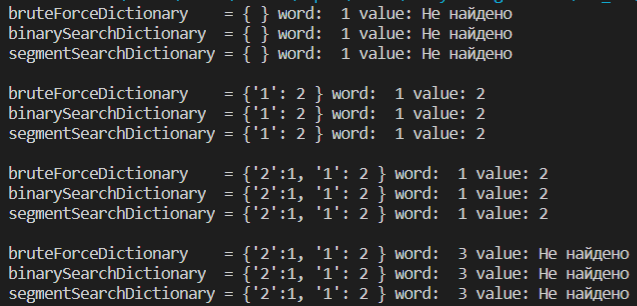
\includegraphics[scale=0.9]{testing.png}
            \caption{Результаты тестирования алгоритмов.}
            \label{png:testing:result}
        \end{figure}
\newpage